
\subsubsection{The Einfeldt Problem}\label{ss:einfeldt}

In 1986  Einfeldt, \textit{et al.}~\cite{einfeldt}  studied Riemann problems using Godunov's method near low densities. Referring to Figure~\ref{fig:shockTube} the domain  $[x |  -0.5 \le x \le 0.5]$ has  a diaphragm at $x = 0.$ and is filled with ideal gases with $\gamma = 1.4$, density $\rho = 1$, and total energy per unit volume $E = 3$ on both sides, but with x-momentum on the left $m_{l_1} = -2$ and on the right $m_{r_1} = 2$ (with $m_{r_{23}} = m_{l_{23}} = 0$) , creating, as time passes, a region of very low density near the diaphragm.  This is sometimes refered to as the \textit{1,2,3-problem} since the initial state has $[\rho, |m_i|, E] = [1, 2, 3].$ The input decks for hopr and flexi are listed in the \ref{ssec:hoprin-einfeldt} and \ref{ssec:flexiin-einfeldt}.  The results at $t = 0.05$ for primitive variables are shown in Figure~\ref{fig:PVmulti123} and for conserved variables in Figure~\ref{fig:multi123}

\begin{table}[h!]
 \begin{center}
  \caption{Initial conditions for Einfeldt's test case.}
  \label{tab:einfeldtIC}
  \begin{tabular}{|c|ccc|cccc|cccc|} \hline
   \textbf{Case} & \multicolumn{3}{c|}{\textbf{Domain}} & \multicolumn{4}{c|}{\textbf{Left Gas}} & \multicolumn{4}{c|}{\textbf{Right Gas}} \\ \hline
   \multirow{2}{*}{$123$} & $x_L$ & $x_D$ & $x_R$ & $\rho$ & $u$ & $P$ & $\gamma$ & $\rho$ & $u$ & $P$ & $\gamma$ \\ \cline{2-12}
   \multicolumn{1}{|c|}{} & 0. & 0.5 & 1.  & 1. & -2. & 0.4 & 1.4 & 1. & 2. & 0.4 & 1.4 \\ \hline
  \end{tabular}
 \end{center}
\end{table}

\begin{figure}[h!]
 \centering
 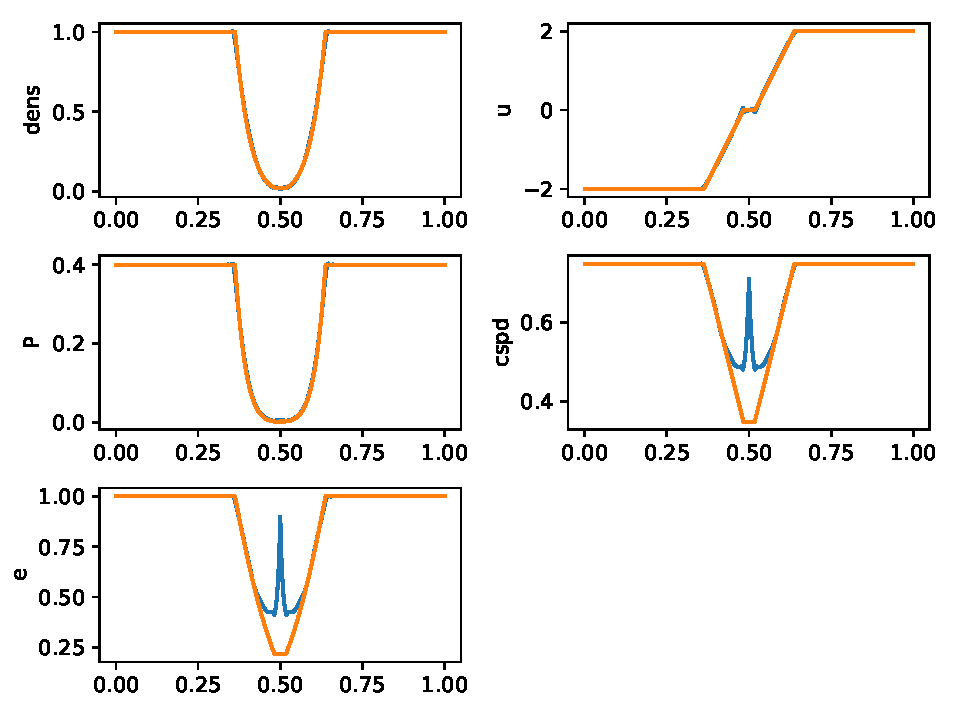
\includegraphics[scale=0.8]{figures/einfeldt-PV.pdf}
 \caption{Einfeldt problem at $t = 0.05$ with 100 equal sized elements in the $x$-direction, but showing the conserved density and the primitive variables: specific internal energy, x-velocity, pressure, and sound speed.  These data reflect the slight oscillation of the very low density region near the diaphragm. Each of these primitive variables are computed using density as a divisor causing large deviations in those variables. Exact data are the blue curves.}
 \label{fig:PVmulti123}
\end{figure}

\begin{figure}[h!]
 \centering
 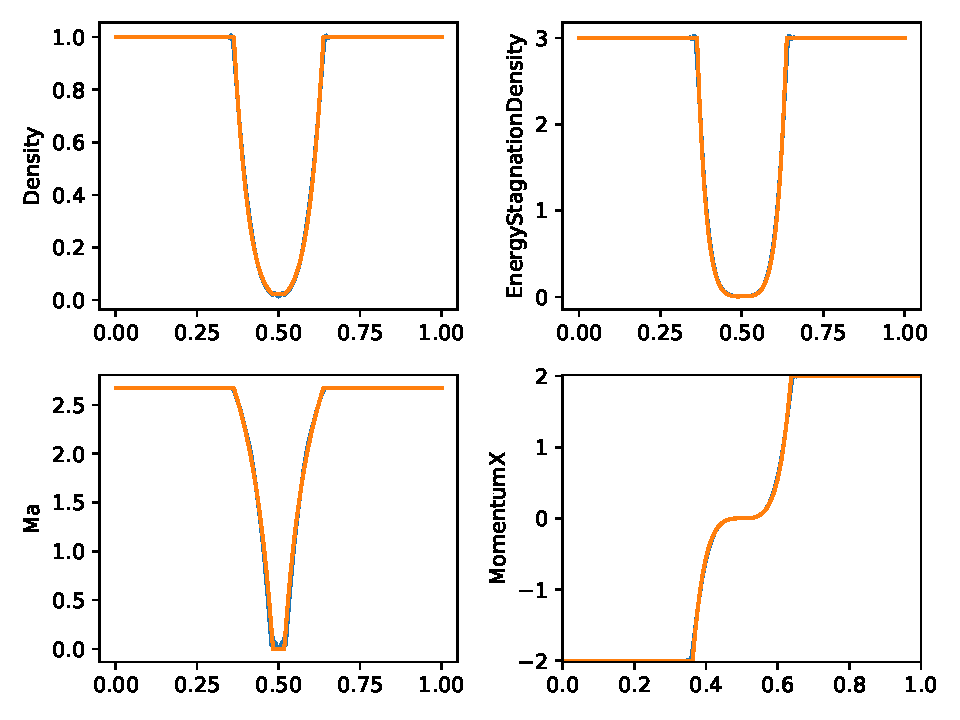
\includegraphics[scale=0.8]{figures/einfeldt-CV.pdf}
 \caption{Einfeldt problem at $t = 0.05$ with 100 equal sized elements in the $x$-direction; showing conserved Flexi variables (blue curves) compared to the exact solution (red curves).}
 \label{fig:multi123}
\end{figure}


Tables~\ref{tab:123Eps} shows the average error for the Flexi solution is less than $0.0016$ with conserved variables being much closer to the exact solution.

\begin{table}[h!]
 \centering
 \begin{tabular}{|c|c|} \hline
   Variable & $\bar{\epsilon}$ \\ \hline \hline
   $\rho$ & 4.7E-4 \\
   $m_x$  & 7.2E-4 \\
   $E$      & 9.3E-4 \\ \hline
   $v_x$  & 6.4E-4 \\
   $u$     & 1.59E-3 \\
   $P$     & 3.2E-4 \\ \hline
 \end{tabular}
 \caption{Average error (\textit{c.f.,} Eq.~\ref{eq:error}) for the Einfeldt Problem}\label{tab:123Eps}
\end{table}

\paragraph{Conclusions}
Flexi results for the Einfeldt problem match very well with the exact solution for conserved variables, although the density near the diaphragm shows oscillations. Any derived variable having density will reflect large discrepancies in that region due to division by very small numbers.
